\documentclass[11pt]{article}
\ifdefined\pdftrailerid\pdftrailerid{}\fi
\ifdefined\pdfinfoomitdate\pdfinfoomitdate=1\fi
\usepackage[T1]{fontenc}
\usepackage{lmodern,amsmath,amssymb,amsthm,mathtools,microtype,booktabs}
\usepackage[margin=1in]{geometry}
\usepackage{xcolor,tikz,needspace}
\usepackage{xurl}
\usetikzlibrary{arrows.meta,positioning}
\usepackage[colorlinks=true,linkcolor=blue!50!black,citecolor=blue!50!black,urlcolor=blue!50!black]{hyperref}
\hypersetup{pdftitle={A Fixed Particle Test for Computation in a Forced Viscous Flow},pdfauthor={OpenAI}}
\newtheorem{theorem}{Theorem}
\newtheorem{lemma}{Lemma}
\newtheorem{corollary}{Corollary}
\newcommand{\T}{\mathbb T}
\newcommand{\R}{\mathbb R}
\newcommand{\N}{\mathbb N}
\newcommand{\Z}{\mathbb Z}
\DeclareMathOperator{\diver}{div}
\DeclareMathOperator{\supp}{supp}
\title{A Fixed Particle Test for Computation\\ in a Forced Viscous Flow}
\author{OpenAI}
\date{September 27, 2026}
\begin{document}
\maketitle
\begin{abstract}
We construct smooth external forces for incompressible Navier--Stokes flow
on a fixed flat three-torus at any fixed positive computable viscosity,
from zero initial velocity, such that a fixed
particle enters a fixed open set exactly when a prescribed Turing machine
halts. Every mixed derivative of the force and velocity is bounded and
square-integrable in time in spatial supremum norm. The construction uses
the machine's ordinary instructions, records their history in a third
coordinate, and compensates for finer spatial gates by longer time steps.
\end{abstract}

\section{Introduction}\label{sec:introduction}

Fix a flat three-dimensional torus, a positive viscosity, zero initial
fluid velocity, one particle label, and an open region that serves as a
detector. Can a finite program for an external force make that particle
enter the region exactly when a given Turing machine halts? The machine
and its finite input may change the force; the geometry, initial velocity,
particle label and detector remain fixed. We prove this for an explicit
family of smooth forces. The resulting reachability problem is undecidable.

The question connects computability with the dynamics of a continuous
system. Turing proved that no machine can decide whether an arbitrary
described machine ever prints a designated symbol \cite[Section~8]{Turing}.
The halting formulation used here follows by a finite modification
that halts on that event. A bounded
continuous phase space can represent such a tape by an infinite positional
expansion. Moore's generalized shifts made this connection explicit:
local symbol changes and shifts of the tape become affine operations on
real coordinates \cite{Moore1990,Moore}. Exact real coordinates supply the unbounded
information capacity; this is not a bound on what a finite-precision
measurement can recover.

A further issue arises when such operations are realized by a smooth
flow. A machine may overwrite a symbol or merge two states, whereas the
flow between two finite times is invertible. Retaining intermediate
information is a classical way to avoid this loss \cite[Section~3]{Landauer}.
Bennett gave an explicit reversible simulation that records the index of
each executed instruction on a history tape \cite[Eqs.~(9)--(11)]{Bennett}. Our construction
uses the same information-retention principle in a different setting:
a third real coordinate retains the selected branches, while two planar
coordinates execute the original, possibly irreversible machine.

Computational universality has also been realized in fluid trajectories.
Cardona, Miranda, Peralta-Salas and Presas constructed stationary Euler
flows on an adapted Riemannian three-sphere whose trajectories simulate
Turing machines \cite{CMPP}. Their proof passes through area-preserving
realizations of generalized shifts. Dyhr, Gonz\'alez-Prieto, Miranda and
Peralta-Salas subsequently obtained stationary unforced Navier--Stokes universality
using an adapted metric and Hodge viscosity \cite{DGMP}. Their velocity
is harmonic for the chosen Hodge Laplacian, so the viscous term vanishes.

Fixed-metric computation also has precedents. Cardona, Miranda and
Peralta-Salas construct universal steady Euler flows on Euclidean $\R^3$
with infinite energy, and robust tape-bounded simulations on the flat
three-torus, observed before exit from a prescribed compact region
\cite[arXiv version~3, Theorems~1 and~26]{CMPBeltrami}.
Their unforced viscous version starts from nonzero Beltrami velocity
and traverses a finite interval of its Euler trajectory, chosen to cover
the bounded computation \cite[arXiv version~3, Remark~29]{CMPBeltrami}.

Here the flat torus and viscosity are fixed in advance and the fluid
starts at rest. The
machine and input instead enter an external force prescription. These
are different choices of data for the fluid equation, and the earlier
results do not supply the construction below.

There is an elementary way to force a chosen smooth incompressible
velocity: subtract its viscous term from its material acceleration.
The mathematical work lies in choosing that velocity from the finite
instruction table. It must execute each instruction, retain the information
needed for invertibility, and avoid the detector at every intermediate
time of a nonhalting run. In particular, our force formula must prescribe
all instruction branches; it must not first execute the input computation
and then replay its trajectory.

We implement an instruction in two pulses. The first records its branch
number in the third coordinate. The second reads the newest record through
a periodic gate and applies the corresponding planar motion. Earlier
records remain present but do not affect that gate. As the history grows,
the gates have finer spatial scales. We make successive steps longer so
that the time-dependent velocity and force have square-integrable
derivatives of every fixed order.

The result concerns exact material trajectories for these explicitly
constructed forces. It gives neither a uniform perturbation tolerance
for arbitrarily long runs nor an efficient simulation-time bound. Its
existence and uniqueness proof uses the prescribed smooth velocity;
it is not a regularity theorem for general Navier--Stokes data.

\section{The statement and the history invariant}\label{sec:statement}

Write $\T=\R/\Z$ and fix a positive computable viscosity $\nu$.
For velocity $u(t,X)$, pressure $p(t,X)$ and external force $f(t,X)$,
the incompressible Navier--Stokes equations are
\begin{equation}\label{eq:NS}
 \partial_tu+(u\cdot\nabla)u=-\nabla p+\nu\Delta u+f,
 \qquad \diver u=0,\qquad u(0)=0
\end{equation}
on the unit flat torus $\T^3$. Pressure is periodic and has mean zero.
We write $X=(x,y,z)$ for a spatial point, use representatives in $[0,1)$
when specifying a coordinate interval, and take $\|\cdot\|_\infty$ over
space. The material flow of a smooth velocity $u$ is defined by
\[
 \frac{d}{dt}\Phi_u(t,a)=u(t,\Phi_u(t,a)),\qquad \Phi_u(0,a)=a.
\]
For a label $a_*\in\T^3$ and an open set $O\subset\T^3$, the
particle event is $\Phi_u(t,a_*)\in O$ for some finite $t$.

An effective force prescription is a finite program that evaluates the
force and any requested mixed derivative at computably supplied space-time
arguments, to any prescribed rational error. It also supplies the derivative
bounds on compact sets used below. The program prescribes the transition
mechanism on all its branches; it does not compute and replay the
distinguished execution. No running-time bound is required.

A classical competitor has continuous velocity, spatial derivatives through
order two, time derivative, pressure and pressure gradient on every closed
cylinder $[0,T]\times\T^3$, with the periodicity and pressure normalization
above. The constructed solution is smooth, including all one-sided time
derivatives at zero.

\Needspace{23\baselineskip}
\begin{theorem}\label{thm:main}
There is an algorithm taking a deterministic single-tape machine $M$ and
a finite word $w$ to an effective smooth mean-zero force $f_{M,w}$ for
\eqref{eq:NS}, with the following properties.
\begin{enumerate}
\item The equation has a global smooth solution $u_{M,w}$, unique among
classical solutions on every finite time interval.
\item For every time order $h\geq0$ and spatial multi-index $\mu$, both
\[
 t\longmapsto\|\partial_t^h\partial_X^\mu u_{M,w}(t)\|_\infty,
 \qquad
 t\longmapsto\|\partial_t^h\partial_X^\mu f_{M,w}(t)\|_\infty
\]
belong to $L^\infty(0,\infty)\cap L^2(0,\infty)$.
\item The particle initially at $a_*=(1/8,3/8,0)$ enters
\[
 O=\{(x,y,z)\in\T^3:1/2<x<1\}
\]
at a finite time if and only if $M$ halts on $w$.
\end{enumerate}
The force may additionally be chosen divergence free, with unchanged
velocity and observation. Constants in the derivative estimates may
depend on $M,w,\nu$ and the derivative orders. After a loading interval,
the prescribed velocity mechanism depends on $M$ but not on $w$.
\end{theorem}

The proof has one particularly useful invariant. A branch specifies the
current state and the symbols read by one local instruction; the precise
list is given in Section~\ref{sec:planar}. Number these finitely many branches by $1,\ldots,J$ and put $\Lambda=J+1$.
If the first $n$ selected branches are $j_0,\ldots,j_{n-1}$, we will arrange
\begin{equation}\label{eq:history}
 z_n=\sum_{i<n}j_i\Lambda^{-i-1}.
\end{equation}
Thus $\Lambda^n z_n$ is an integer. Translating $z$ by
$j_n\Lambda^{-n-1}$ makes its new value satisfy
\begin{equation}\label{eq:selector}
 \Lambda^n z=\frac{j_n}{\Lambda}\pmod 1.
\end{equation}
A smooth periodic gate can now select instruction $j_n$. This is the
continuous history record corresponding to the transition-index record
in Bennett's reversible simulation \cite{Bennett}. The earlier
digits have become an integer and do not affect this gate. They have not
been erased: they remain in $z$, so two planar updates with overlapping
images can still represent different pasts.

We next construct the planar branches and then realize
\eqref{eq:history} by a divergence-free field. The symbols $j_n$ describe
the trajectory in the proof; they will not occur in the formula for the
force.

Here is the route through the proof. Section~\ref{sec:planar} converts each
instruction into an area-preserving planar motion and proves that it cannot
cause a false detection between nonhalting configurations.
Section~\ref{sec:recording} combines the recorder and these motions into one
smooth incompressible velocity, and proves the event equivalence.
Section~\ref{sec:force} chooses the force, establishes the derivative bounds
and uniqueness, and verifies effective evaluation without running the
machine. The Fourier projection there gives the optional solenoidal force.

A force that eventually stops changing in time poses a further question:
its spatial mechanism must keep computing without progressively changing
the gates. A separate companion gives that finite spatial mechanism
and proves eventual stationarity \cite{Stationary}. The present
proof uses the ordinary machine directly and requires no result
from that companion.

The optional comparison theorem in Appendix~\ref{app:comparison}
also applies on $\R^3$ and $\R^2\times\T$, with explicit Sobolev
and pressure assumptions for other constructed flows. The particle theorem above concerns $\T^3$ only.
For a positive viscosity that is not assumed computable, the same formulas
and estimates hold, with effective evaluation relative to the ability to
approximate that fixed viscosity. Unqualified algorithmic assertions in
this paper use the computable viscosity fixed above.

\section{A machine instruction as a planar motion}\label{sec:planar}

Our task in this section is to turn each machine instruction into a planar
motion whose entire path respects the detector. First encode the tape,
then interpolate the resulting affine update by a Hamiltonian field.

First merge designated halting states into a single state $q_h$, or
adjoin an unreachable $q_h$ if none is designated. Let $Q$ now have
$N\geq1$ states, and let the tape alphabet $\Sigma$ have $m\geq1$
letters, including a blank $\square$. Replace a missing instruction
on symbol $a$ by $(q_h,a,S)$, and give $q_h$ stationary identity
instructions. This finite normalization preserves the halting event,
including an initially halted input. The tape is a sequence $(s_i)_{i\in\Z}$ in $\Sigma$, with finitely many
nonblank cells initially. Place the input word starting at cell zero,
put blanks elsewhere, and start the head at zero in the machine's initial
state. Write
$\delta(q,a)=(q',b,D)$, where $D$ is a left move, right move or stay.

The positional coding is the generalized-shift representation of a tape
\cite[Section~1, Lemma~0]{Moore}, with gaps inserted between symbol intervals.
Give the letters the odd digits $d_a\in\{1,3,\ldots,2m-1\}$ in base
$B=2m+1$, and set
\[
 v(a_0a_1\ldots)=\sum_{r\geq0}d_{a_r}B^{-r-1},
 \qquad I_a=[d_a/B,(d_a+1)/B].
\]
The intervals $I_a$ are separated by gaps of length at least $1/B$.
A code lies in the interval of its first letter, and
$Bv(a\omega)-d_a=v(\omega)$ removes that letter. This proves unique
decoding. A blank tail has value $d_{\square}/(B-1)$, so all initial
codes are rational.

If the head is at cell $k$, encode the two relative tape halves by
\[
 \ell=v(s_{k-1}s_{k-2}\ldots),\qquad r=v(s_ks_{k+1}\ldots).
\]
Put $\kappa=(16N)^{-1}$ and $y_0=3/8$. Enumerate nonhalting states as
$q_0,\ldots,q_{N-2}$ and choose
\[
 c(q_i)=1/8+2i\kappa,\qquad c(q_h)=3/4.
\]
The planar code is $P=(c(q)+\kappa\ell,y_0+\kappa r)$. The state box
$[c(q),c(q)+\kappa]\times[y_0,y_0+\kappa]$ lies in
\[
 K=[1/8,13/16]\times[3/8,7/16].
\]
Every nonhalting state box has $x\leq1/4$; the halting box has $x\geq3/4$.
These inequalities leave room for a fixed detector between the two.

Index the triples $j=(q,l,a)$ by $1,\ldots,J=Nm^2$. Here $a$ is the
letter under the head and $l$ the letter immediately to its left. Their
closed source rectangles are
\[
 R_j=(c(q)+\kappa I_l)\times(y_0+\kappa I_a).
\]
They are pairwise disjoint. If $\ell_*=B\ell-d_l$ and $r_*=Br-d_a$,
the tape instruction is exactly
\begin{equation}\label{eq:branches}
\begin{array}{c|cc}
D&\ell'&r'\\ \hline
R&(d_b+\ell)/B&r_*\\
L&\ell_*&[d_l+(d_b+r_*)/B]/B\\
S&\ell&(d_b+r_*)/B.
\end{array}
\end{equation}
For example, a right move prefixes the written letter $b$ to the left
tape and removes $a$ from the right tape. A left move removes $l$ from
the left tape and prefixes $l,b$ to the old right tail. These operations
explain both entries in each row of the table.

Let $F_j$ be the resulting affine map in the physical coordinates $P$.
It maps the whole rectangle $R_j$ into the next state box, and its linear
part is $\operatorname{diag}(\lambda_j,\lambda_j^{-1})$, with
$\lambda_j=B^{-1},B,1$ respectively. Different image rectangles may
overlap. We will distinguish them by history, not by assuming that an
ordinary machine is reversible.

We have obtained the correct endpoint update. We now realize it by a
continuous motion, keeping every nonhalting-to-nonhalting path to the
left of the detector. Local area-preserving realizations of bijective generalized
shifts also occur in \cite[Proposition~5.1]{CMPP}; here a separate history
coordinate will distinguish different branches with overlapping images.

\Needspace{9\baselineskip}
Let $C_j^0,C_j^1$ be the centers of $R_j,F_j(R_j)$ and
$E_j=C_j^1-C_j^0$. For $0\leq s\leq1$ define
\[
 C_j(s)=C_j^0+sE_j,\quad g_j(s)=1-s+s\lambda_j,
 \quad \gamma_j(s)=\frac{\lambda_j-1}{g_j(s)},
\]
\begin{equation}\label{eq:path}
 \Psi_{j,s}(P)=C_j(s)+
 \operatorname{diag}(g_j(s),g_j(s)^{-1})(P-C_j^0).
\end{equation}
This path starts at $P$ and ends at $F_j(P)$. Its first coordinate is
the convex combination of the two endpoint coordinates. To control the
second coordinate, let $a$ be the source rectangle's vertical half-width.
Convexity of the reciprocal gives
\[
 \frac{a}{g_j(s)}\leq(1-s)a+s\frac{a}{\lambda_j}.
\]
Together with the linear motion of the center, this keeps the entire
rectangle in $K$. In particular, an instruction with nonhalting source
and target stays in $x\leq1/4$ throughout its motion.

Choose a smooth cutoff $\chi$ equal to one on a neighborhood of $K$
and supported in the open unit square. Periodize the compactly supported
Hamiltonian
\[
 H_j(s,x,y)=\chi(x,y)\bigl[
 E_{j,x}(y-C_{j,y}(s))-E_{j,y}(x-C_{j,x}(s))
 +\gamma_j(s)(x-C_{j,x}(s))(y-C_{j,y}(s))\bigr].
\]
The planar field $V_j=(\partial_yH_j,-\partial_xH_j)$ is divergence
free and has mean zero. On the moving rectangle its components are
$E_{j,x}+\gamma_j(x-C_{j,x})$ and
$E_{j,y}-\gamma_j(y-C_{j,y})$. Differentiating \eqref{eq:path} gives
exactly these velocities. Uniqueness for the smooth ODE therefore shows
that $V_j$ realizes the claimed path, including its intermediate-time
bound. The cutoff introduces no error there because all its derivatives
vanish on that path.

\section{Recording and selecting the instruction}\label{sec:recording}

Each instruction uses two pulses. The first reads the current source
rectangle and adds its branch number to the history; the second uses that
new digit to select the planar motion. Thus we can use the individual
motions of Section~\ref{sec:planar} even when their planar images overlap.
Figure~\ref{fig:pulses} shows one step; the formulas below implement it
simultaneously for every possible branch.

\begin{figure}[ht]
\centering
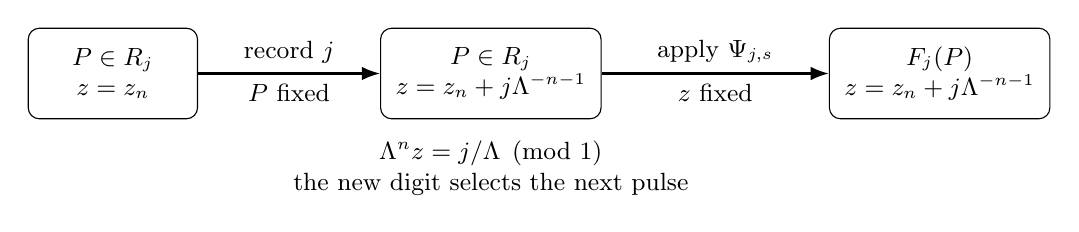
\begin{tikzpicture}[>=Latex,font=\small]
\node[draw,rounded corners,align=center,minimum width=2.15cm,minimum height=1.15cm] (start) at (0,0)
 {$P\in R_j$\\$z=z_n$};
\node[draw,rounded corners,align=center,minimum width=2.8cm,minimum height=1.15cm] (record) at (4.8,0)
 {$P\in R_j$\\$z=z_n+j\Lambda^{-n-1}$};
\node[draw,rounded corners,align=center,minimum width=2.8cm,minimum height=1.15cm] (end) at (10.5,0)
 {$F_j(P)$\\$z=z_n+j\Lambda^{-n-1}$};
\draw[->,thick] (start) -- node[above,align=center] {record $j$} node[below] {$P$ fixed} (record);
\draw[->,thick] (record) -- node[above] {apply $\Psi_{j,s}$} node[below] {$z$ fixed} (end);
\node[align=center] at (4.8,-1.2)
 {$\Lambda^n z=j/\Lambda\pmod 1$\\the new digit selects the next pulse};
\end{tikzpicture}
\caption{One simulated instruction, schematically. The first pulse leaves
both tape coordinates fixed while recording the selected branch. The
second leaves the history fixed while executing that branch's planar
motion. The diagram describes the encoded particle; planar images of
different branches need not be disjoint.}
\label{fig:pulses}
\end{figure}

We specify the cutoffs to ensure that closed rectangle boundaries are
covered. Let
\[
 \rho(s)=\begin{cases}e^{-1/s},&s>0,\\0,&s\leq0,\end{cases}
 \qquad \sigma(s)=\frac{\rho(s)}{\rho(s)+\rho(1-s)}.
\]
For a closed interval $I=[a,b]$, set
\[
 \eta_I^\varepsilon(v)=
 \sigma\!\left(\frac{2(v-a+\varepsilon)}{\varepsilon}\right)
 \sigma\!\left(\frac{2(b+\varepsilon-v)}{\varepsilon}\right).
\]
The cutoff $\eta_I^\varepsilon$ equals one on a neighborhood of $I$
and vanishes outside its $\varepsilon$ enlargement. Products define
the analogous rectangle cutoffs. For the earlier Hamiltonians, choose
$\chi=\eta_K^{1/32}$; its support is strictly inside the unit square.

The source rectangles have gaps at least $\kappa/B$, so the supports in
\[
 G_0(x,y)=\sum_{j=1}^Jj\eta_{R_j}^{\kappa/(4B)}(x,y)
\]
are disjoint. Periodize this function from the unit-square chart and put
\[
 G(x,y)=G_0(x,y)-G_0(x,y-1/2).
\]
The original supports lie in $1/4<y<1/2$; their half-period translates
miss every $R_j$. Consequently $G=j$ on $R_j$ and $G$ has zero mean.
The correction permits a mean-zero vertical recorder without altering
the tracked computation. Define the gates by periodizing the following
bumps with period one:
\[
 b_j(z)=\eta_{\{j/\Lambda\}}^{1/(4\Lambda)}(z),
 \qquad \Lambda=J+1.
\]
Their supports are disjoint and each equals one near its own center.

Let $\theta(s)=\sigma(2s-1/2)$. It rises smoothly from zero to one
inside $(0,1)$ and is constant near both endpoints. Set
\[
 S_n=2^{n^2},\quad t_0=1,\quad t_{n+1}=t_n+2S_n,
 \qquad
 \alpha_n(t)=\frac{t-t_n}{S_n},\quad
 \beta_n(t)=\frac{t-t_n-S_n}{S_n}.
\]
Step $n$ has a recorder interval and an equally long planar interval.

The initial planar code $P_{\rm in}$ is rational. Let $V_{\rm load}$
be the Hamiltonian field of
\[
 \chi(x,y)[(P_{{\rm in},x}-1/8)y-(P_{{\rm in},y}-3/8)x].
\]
It translates $(1/8,3/8)$ along its straight segment to $P_{\rm in}$.
Define the velocity on $[0,\infty)\times\T^3$ by
\begin{equation}\label{eq:field}
\begin{split}
 U(t,x,y,z)={}&(\theta'(t)V_{\rm load}(x,y),0)\\
 &+\sum_{n\geq0}\left(
 \frac{\theta'(\beta_n(t))}{S_n}
 \sum_{j=1}^J b_j(\Lambda^n z)
 V_j(\theta(\beta_n(t)),x,y),\quad
 \frac{\theta'(\alpha_n(t))}{S_n\Lambda^{n+1}}G(x,y)
 \right).
\end{split}
\end{equation}
The displayed sum is a formula for all possible instructions. It has no
reference to which instruction the machine will actually select.

At any time only one stage can be active. Since $t_n\geq1+2n$, the sum
is locally finite; the zero collars make every join smooth. Multiplying
a planar divergence-free field by a function of $z$ preserves its planar
divergence, and the vertical component is independent of $z$. Thus
$\diver U=0$. Each planar field has zero planar mean, while $G$ has
zero planar mean, so $U$ has zero spatial mean. Also $U(0)=0$.

After the loader, the particle has planar coordinate $P_{\rm in}$ and
$z_0=0$. Suppose at $t_n$ it has the current planar configuration and
history \eqref{eq:history}. It belongs to exactly one source rectangle,
say $R_{j_n}$. During the recorder interval its planar coordinate stays
fixed, while integration of the last component in \eqref{eq:field}
adds $j_n\Lambda^{-n-1}$ to $z$. Equation \eqref{eq:selector} follows.
On the planar interval only $b_{j_n}$ is nonzero at this particle, and
its value is one. Its path is therefore
$\Psi_{j_n,\theta(\beta_n(t))}(P(t_n))$, ending at the next machine code.
The third coordinate stays fixed on this interval. This proves the
induction and \eqref{eq:history} for every $n$.

There is no wraparound ambiguity for the tracked history:
$0\leq z_n\leq1-\Lambda^{-n}$. At a known step its finite radix
expansion recovers every previous branch, hence every head displacement
and the absolute head position. The planar coordinates recover the
state and relative tape. This is an encoding of the computation, not
merely a halting indicator.

If the machine halts, a planar code with $x\geq3/4$ is reached after
finitely many finite stages. If it is initially halted, the loader
already reaches such a code. Conversely, for a nonhalting run the loader
stays in $x\leq1/4$, a recorder interval does not change $x$, and
\eqref{eq:path} stays in $x\leq1/4$ at every planar stage. This proves
both directions of the event equivalence at every real time.

\section{Slowing the gates and obtaining the force}\label{sec:force}

The velocity now implements the machine and gives the correct event at
every time. It remains to control its derivatives, realize it as the unique
fluid velocity, and show that the force has a finite effective prescription.

\subsection{Bounds for the prescribed velocity}

Why choose the rapidly growing stage lengths $S_n$? Differentiating a
gate $b_j(\Lambda^n z)$ $k$ times costs a factor $\Lambda^{nk}$.
The factor $S_n^{-1}$ in the velocity compensates for this at every
fixed derivative order. More precisely, for a time order $h$ and
spatial multi-index $\mu=(\mu_x,\mu_y,\mu_z)$, the fixed smooth
profiles above give, throughout step $n$,
\begin{equation}\label{eq:bounds}
 \|\partial_t^h\partial_X^\mu U(t)\|_\infty
 \leq C_{h,\mu}S_n^{-1-h}\Lambda^{n\mu_z}.
\end{equation}
The profiles $V_j$ and their phase derivatives are uniformly bounded
for $0\leq s\leq1$, because $g_j(s)>0$. The recorder has no $z$
dependence and has an additional small factor $\Lambda^{-n-1}$, so it
also satisfies this estimate. The constants depend on the finite table
and derivative orders but not on $n$.

The right side of \eqref{eq:bounds} is bounded, and integration over
the two intervals of length $S_n$ gives
\[
 \int_1^\infty
 \|\partial_t^h\partial_X^\mu U(t)\|_\infty^2\,dt
 \leq 2C_{h,\mu}^2\sum_{n\geq0}
 2^{-(1+2h)n^2}\Lambda^{2n\mu_z}<\infty.
\]
The loader occupies a compact time interval and adds a finite amount.
Now prescribe
\begin{equation}\label{eq:force}
 f=\partial_tU+(U\cdot\nabla)U-\nu\Delta U.
\end{equation}
Then $(u,p)=(U,0)$ solves \eqref{eq:NS}. Every mixed derivative of $f$
is a finite sum of derivatives of $U$ and products of two such
derivatives. Each factor is bounded, and each has the stated temporal
$L^2$ norm; use one bounded factor and one $L^2$ factor in a product.
All force estimates in the theorem follow. Integration of
\eqref{eq:force} over the torus gives zero mean, because $U$ has zero
mean and $(U\cdot\nabla)U=\diver(U\otimes U)$.

\subsection{Uniqueness for the constructed torus flow}
The residual identity gives the solution. We now show that its particle
event is determined by the force and initial data. The proof is the
classical difference-energy comparison \cite[Section~18]{Leray}.
If $(v,p)$ is another solution in the classical class of
Section~\ref{sec:statement}, set $w=v-U$. Subtraction gives
\[
 w_t+(v\cdot\nabla)w+(w\cdot\nabla)U
  =-\nabla p+\nu\Delta w,\qquad \diver w=0.
\]
Multiplication by $w$ and periodic integration by parts yield
\[
 \frac12\frac{d}{dt}\|w\|_2^2+\nu\|\nabla w\|_2^2
 \leq\|\nabla U\|_{\infty,\mathrm{op}}\|w\|_2^2.
\]
The stated continuity of $v_t$, the first two spatial derivatives and
pressure gradient justifies all these operations. The transport and
pressure terms vanish by incompressibility. Boundedness of $\nabla U$
on each finite interval and $w(0)=0$ give $w=0$ by Gronwall's
inequality. The equation then gives $\nabla p=0$, and mean-zero
normalization gives $p=0$. Smoothness and bounded spatial gradient on
the compact torus give a unique material flow through every finite
time. Thus the event already proved for $U$ belongs to the unique
fluid solution. Appendix~\ref{app:comparison} supplies the corresponding
noncompact comparison theorem and the finite-time flow identities.

\subsection{Solenoidal forcing with the same velocity}
The Helmholtz--Leray projection removes the divergence of the force.
Because it changes a gradient, it also changes the pressure. The
following quantitative version is useful both for the present
$L^2$ bounds and for other time profiles.

\begin{lemma}[Effective periodic projection]\label{lem:projection}
Let $g$ be a smooth mean-zero vector field on
$[0,\infty)\times\T^3$, effectively evaluable together with all
mixed derivatives and with effective bounds for those derivatives
on every finite time interval. There is a unique smooth mean-zero
$\phi$ satisfying $\Delta\phi=\diver g$. Both $\phi$ and
$g_{\rm sol}=g-\nabla\phi$ are effective, and $g_{\rm sol}$ is
divergence free and mean zero. For every $h\geq0$ and spatial
multi-index $\mu$,
\begin{equation}\label{eq:projection-estimate}
 \|\partial_t^h\partial_X^\mu\nabla\phi(t)\|_\infty
 \leq C_\mu\max_{1\leq i\leq3}
 \|\partial_t^h\partial_{X_i}^{|\mu|+5}g(t)\|_\infty.
\end{equation}
Thus, when all mixed derivatives of $g$ are bounded, square-integrable
in time in spatial supremum norm, or rapidly decaying, the same
property holds for $g_{\rm sol}$. Here rapid decay means a finite
supremum after multiplication by $(1+t)^A$, for every $A\geq0$ and
every fixed derivative order. Time periodicity and stationarity
after a given time are also preserved. If $(U,P)$ solves the equation
with force $g$, then it solves it with force $g_{\rm sol}$ and
pressure $P-\phi$.
More precisely, any common pointwise time weight on the finitely many
derivatives on the right of \eqref{eq:projection-estimate} passes to
the derivative on its left. Thus a specified polynomial bound is
preserved whenever those higher spatial derivatives have that bound.
\end{lemma}
\begin{proof}
For the Fourier basis $e^{2\pi i k\cdot X}$ set
\[
 \widehat\phi(k)=-\frac{i k\cdot\widehat g(k)}{2\pi|k|^2}
 \quad(k\ne0),\qquad \widehat\phi(0)=0.
\]
The multiplier for $\nabla\phi$ is $kk^{\mathsf T}/|k|^2$,
whose operator norm is one. For a derivative of order $r$, integrate
the coefficients of $\partial_t^hg$ by parts $r+5$ times in a
coordinate with maximal $|k_i|$. A term of the differentiated series
is bounded by a fixed multiple of $|k|^{-5}$ times the right-hand
derivative norm in \eqref{eq:projection-estimate}. There are
$O(n^2)$ points in the shell $\|k\|_\infty=n$. The series and its
derivatives therefore converge absolutely, with an explicit tail
bounded by $C\sum_{n>K}n^{-3}$. The series for $\phi$ has one
further factor $|k|^{-1}$. Termwise differentiation proves the
Poisson equation; the Fourier coefficients also prove uniqueness
among mean-zero solutions and establish
\eqref{eq:projection-estimate}.

The Fourier identification used here is justified in
Appendix~\ref{app:fourier}. Since $g$ is real,
$\widehat\phi(-k)=\overline{\widehat\phi(k)}$, so $\phi$ is real.

Riemann sums with a bound on one more spatial derivative compute
each coefficient to any requested error. Combined with the tail
estimate, this gives effective evaluation of every derivative.
The estimate is pointwise in time and commutes with time
derivatives, so it proves each stated norm and weighted-decay
assertion. Linearity and uniqueness of the mean-zero Poisson
solution preserve periodicity and eventual stationarity. Finally,
\[
 -\nabla(P-\phi)+(g-\nabla\phi)=-\nabla P+g,
\]
which proves the pressure formula.
Conversely, a classical solution with force $g_{\rm sol}$ and pressure
$p$ solves the equation with force $g$ and pressure $p+\phi$.
This correspondence preserves the normalized classical class on the
torus, since $\phi$ is smooth and mean zero. It therefore preserves
uniqueness for fixed initial data, as well as the reference velocity.
\end{proof}

To apply Lemma~\ref{lem:projection} to the force in \eqref{eq:force},
we still need to verify its effective-evaluation hypotheses. The next
subsection supplies them and completes the optional solenoidal
construction. This periodic projection does not assert preservation
of compact support on a Euclidean domain, nor does it preserve
pressure zero.

\subsection{Effective evaluation without a simulated execution}


It remains to check that the prescription really is effective. We
record the elementary fact about smooth profiles separately so that
its computational hypothesis is explicit.

\begin{lemma}[Effective smooth profiles]\label{lem:profiles}
The functions $\rho,\sigma$ defined in Section~\ref{sec:recording}
and their finite products, sums, translations, and positive rescalings
by computable parameters have effective evaluations of every derivative,
with effective derivative bounds on compact sets. A reciprocal may be
included when an effective positive lower bound for its denominator is
given. A compactly supported profile periodized through zero collars
has the same property if a rational box containing its support is
supplied. An infinite sum of such profiles has this
property on compact sets if a finite superset of all possibly active
indices can be computed there.
\end{lemma}
\begin{proof}
On $s>0$, derivatives of $\rho$ have the form $P(1/s)e^{-1/s}$,
where $P$ is an effectively computable polynomial. For $v>0$,
$v^m e^{-v}\leq(m+k)!v^{-k}$ bounds every monomial and gives an
effective neighborhood of zero where each derivative is smaller than
a requested error. Away from that neighborhood ordinary effective
arithmetic and the exponential evaluate it. This avoids deciding
whether the supplied real is exactly zero. The denominator of
$\sigma$ is at least $e^{-2}$; quotient differentiation therefore
gives effective bounds as well. The finite operations in the statement
preserve these properties by their differentiation rules.

For a profile $\psi$ with support in a supplied rational interval
$[a,b]$, obtain a rational $q$ with $|s-q|\leq1$. A translate
$\psi(s-k)$ can be nonzero only for an integer
$k\in[q-b-1,q-a+1]$. Evaluating all integers in this rational interval
therefore computes the periodization and each of its derivatives;
no integer-part computation on the real $s$ is required. The same
argument works coordinatewise for a supplied rational box.
A supplied finite active-index
bound reduces the last assertion to a finite sum. Local finiteness
without that effective bound would not suffice for this argument.
\end{proof}

All tables, rational initial codes, affine maps and stage times are
obtained from the finite input. Lemma~\ref{lem:profiles} applies to
their cutoffs and phase functions; the denominators $g_j(s)$ have the
effective positive lower bounds $\min\{1,\lambda_j\}$. The supports
of $\chi$ and the rectangle cutoffs lie in the rational coordinatewise
enlargements of $K$ by $1/32$ and of $R_j$ by $\kappa/(4B)$,
respectively. The unperiodized gate defining $b_j$ is supported in
$[(j-1/4)/\Lambda,(j+1/4)/\Lambda]$. Thus every periodization has
the supplied support enclosure required by the lemma. For a time
argument, obtain a rational
upper bound $T>t$. The inequality $t_n\geq1+2n$ gives a finite superset
of possible active stages in \eqref{eq:field}; evaluating all of them
is sufficient. Periodizations are evaluated by the same finite-superset
procedure in coordinate charts, without deciding a real argument's
integer part. The Gaussian series above gives effective norm bounds:
for example, if $n\geq4\Lambda\mu_z$, then
$\Lambda^{2n\mu_z}\leq2^{n^2/2}$.

We may now apply Lemma~\ref{lem:projection} to $f$ in
\eqref{eq:force}. It gives an effective mean-zero solenoidal force
$f-\nabla\phi$ with solution $(U,-\phi)$, the same derivative bounds,
and the same particle event. The lemma's pressure correspondence
also transfers uniqueness from the original force. Riemann sums
with derivative error bounds compute the Fourier coefficients, and
the summable tail controls truncation. Neither this procedure nor the
raw-force evaluation uses the branch sequence $j_0,j_1,\ldots$.
For $t\geq1$ the loader and all its derivatives vanish, so the raw
force depends on $M$ and $\nu$ but not on $w$. Its spatial projection
at that time has the same independence.
This completes the proof of
Theorem~\ref{thm:main}.

\begin{corollary}
No algorithm decides the fixed particle event for every force description
produced by this construction.
\end{corollary}
\begin{proof}
Compose a proposed decision procedure with the terminating compiler of
Theorem~\ref{thm:main}. The event equivalence would decide whether an
arbitrary machine halts on its finite input. This would also decide
Turing's symbol-printing problem \cite[Section~8]{Turing}: modify the
simulated machine to halt when the specified symbol is printed and
to continue forever otherwise, including if the original machine stops
without printing it. Turing proves that no such decision procedure exists.
Equivalently, one may fix a universal machine and encode the machine
and word in its finite input; the same event then tests its computation.
\end{proof}

\appendix
\section{Comparison on noncompact domains and Fourier identification}
The main particle theorem is already complete. We record two analytic
details separately: a comparison theorem with precise noncompact
pressure assumptions, useful for other prescribed flows, and the
elementary Fourier uniqueness argument used in the periodic projection.

\subsection{The precise comparison class}\label{app:comparison}
Let $\Omega$ be $\T^3$, $\R^3$, or
$\R^2\times\T$. A classical solution on $[0,T]$ has continuous
$u$, $u_t$, all spatial derivatives of $u$ through order two, $p$, and
$\nabla p$ on the closed time cylinder, and satisfies the equation
pointwise. In the noncompact cases we additionally require
\begin{equation}\label{eq:energy-class}
 \begin{gathered}
 u\in C([0,T];H^2(\Omega))\cap C^1([0,T];L^2(\Omega)),
 \qquad p\in C([0,T];H^1(\Omega)),\\
 \sup_{[0,T]\times\Omega}(|u|+|\nabla u|)<\infty.
 \end{gathered}
\end{equation}
The Sobolev spaces are periodic in the torus coordinates. On $\T^3$
the pressure has mean zero; on the noncompact domains its $H^1$
membership fixes the representative, since a nonzero spatial constant
is not in $L^2$.

\begin{lemma}[Prescribed motion and uniqueness]\label{lem:realization}
Fix $\nu>0$ and $\Omega\in\{\T^3,\R^3,\R^2\times\T\}$.
Let $U$ be smooth and divergence free on $[0,\infty)\times\Omega$,
with $U(0)=0$, and suppose $U$ and $\nabla U$ are bounded on every
finite closed time cylinder. In the noncompact cases assume the
velocity conditions in \eqref{eq:energy-class}. Then the force
\[
 \mathcal F_\nu[U]=U_t+(U\cdot\nabla)U-\nu\Delta U
\]
has the solution $(u,p)=(U,0)$, unique in the classical class just
defined on each finite time interval. Its material trajectories exist
uniquely for every finite time. On $\T^3$, mean-zero $U$ gives
mean-zero $\mathcal F_\nu[U]$.

More generally, if an independently constructed pair $(U,P)$ is a
classical solution in the same class for a given force and initial
velocity, it is the unique solution for those data in that class.
In either noncompact uniqueness statement, the competitor's gradient
bound can be omitted while keeping its bounded velocity and all other
conditions. The reference velocity $U$ still has bounded gradient.
For smooth $U$, each finite-time material map $\Phi_t$ is a smooth
diffeomorphism and satisfies
\[
 U(t,\cdot)=(\partial_t\Phi_t)\circ\Phi_t^{-1},\qquad
 \partial_{tt}\Phi_t(a)
   =(f-\nabla P+\nu\Delta U)(t,\Phi_t(a)).
\]
\end{lemma}
\begin{proof}
Substitution proves the residual assertion. For either uniqueness
statement, let $(v,p)$ be another solution for the same data, and set
$w=v-U$ and $q=p-P$. Subtracting the equations gives
\[
 w_t+(v\cdot\nabla)w+(w\cdot\nabla)U
   =-\nabla q+\nu\Delta w,\qquad \diver w=0.
\]
On the torus, multiplication by $w$ and periodic integration give
\begin{equation}\label{eq:energy-comparison}
 \frac12\frac{d}{dt}\|w\|_2^2+\nu\|\nabla w\|_2^2
 \leq\|\nabla U(t)\|_{\infty,\mathrm{op}}\|w\|_2^2.
\end{equation}
The transport and pressure integrals vanish by incompressibility.

Here are the cutoff details on the other two domains. Let $x'$ denote
the noncompact coordinates, choose $0\leq\zeta\leq1$ smooth with
compact support, equal to one on $|x'|\leq1$, and set
$\zeta_R(x')=\zeta(x'/R)$. Multiply the difference equation by
$\zeta_Rw$ and integrate in all coordinates. Integration by parts
leaves, besides the term $-\int\zeta_Rw\cdot(w\cdot\nabla)U$,
three boundary errors. Their absolute values are at most
\[
 \frac C R\|v\|_\infty\|w\|_2^2,\qquad
 \frac C R\|q\|_2\|w\|_2,\qquad
 \frac {C\nu}R\|\nabla w\|_2\|w\|_2,
\]
respectively for transport, pressure, and viscosity. For example,
the pressure term is $\int q\nabla\zeta_R\cdot w$ because
$\diver w=0$. Each displayed norm is uniformly bounded on $[0,T]$
by \eqref{eq:energy-class}. Also $w\in C^1([0,T];L^2)$
justifies differentiating $\int\zeta_R|w|^2$. Integrate the identity
between any two times and then let $R\to\infty$. Dominated
convergence applies to the quadratic terms and the error integrals
tend to zero. This gives \eqref{eq:energy-comparison} in integrated
form, equivalently almost everywhere in time. Thus no decay of the
pressure beyond the stated $C_tH^1$ condition has been assumed.

On every finite interval the coefficient in
\eqref{eq:energy-comparison} is bounded. Its integrating factor and
$w(0)=0$ imply $w=0$. The equation then gives $\nabla q=0$;
the mean-zero or $H^1$ pressure convention gives $q=0$.
The estimates use boundedness of $v$ but never a bound on $\nabla v$,
which proves the stated competitor extension.

Finally, bounded spatial gradient gives a uniformly Lipschitz vector
field on each finite time interval, so the material ODE has unique
local solutions. Bounded velocity prevents escape to infinity in
finite time. Successive local solutions therefore cover each finite
interval, and periodic coordinates descend to their quotients.
Solving the same ODE backwards on $[0,t]$ gives the inverse map.
Smooth dependence on the initial point proves the diffeomorphism
assertion; differentiating the trajectory equation proves the two
displayed identities.
For the mean assertion, integrate the residual: the integrals of
$\Delta U$ and $(U\cdot\nabla)U=\diver(U\otimes U)$ vanish on
the torus.
\end{proof}


\subsection{Identifying continuous periodic functions}\label{app:fourier}
A continuous function on $\T^3$ is determined by its Fourier
coefficients. Here is the approximate-identity argument used in
Lemma~\ref{lem:projection}.

In one variable,
\[
 F_N(s)=\frac1N\left|\sum_{j=0}^{N-1}e^{2\pi i js}\right|^2
\]
is nonnegative, has integral one, and has Fourier coefficients
$(1-|k|/N)_+$. Outside any fixed neighborhood of the integers,
the geometric-sum formula bounds $F_N$ by $C/N$. Hence the product
of three such kernels has mass tending to one in every neighborhood
of zero. Uniform continuity shows that convolution with this product
converges uniformly to any continuous function on $\T^3$.
Vanishing Fourier coefficients therefore imply a vanishing function.


\begin{thebibliography}{99}
\bibitem{Bennett} C.~H. Bennett, Logical reversibility of computation,
\emph{IBM J. Res. Develop.} \textbf{17} (1973), 525--532.
\href{https://doi.org/10.1147/rd.176.0525}{\nolinkurl{doi:10.1147/rd.176.0525}}.

\bibitem{CMPBeltrami} R. Cardona, E. Miranda and D. Peralta-Salas,
Computability and Beltrami fields in Euclidean space,
\emph{J. Math. Pures Appl.} \textbf{169} (2023), 50--81.
\href{https://doi.org/10.1016/j.matpur.2022.11.007}{\nolinkurl{doi:10.1016/j.matpur.2022.11.007}}.
\href{https://arxiv.org/abs/2111.03559v3}{\nolinkurl{arXiv:2111.03559v3}}.

\bibitem{CMPP} R. Cardona, E. Miranda, D. Peralta-Salas and F. Presas,
Constructing Turing complete Euler flows in dimension 3,
\emph{Proc. Natl. Acad. Sci. USA} \textbf{118} (2021), e2026818118.
\href{https://doi.org/10.1073/pnas.2026818118}{\nolinkurl{doi:10.1073/pnas.2026818118}}.

\bibitem{DGMP} S. Dyhr, \'{A}. Gonz\'alez-Prieto, E. Miranda and
D. Peralta-Salas, Turing complete Navier--Stokes steady states via
cosymplectic geometry, \emph{PNAS Nexus} \textbf{5} (2026), pgag131.
\href{https://doi.org/10.1093/pnasnexus/pgag131}{\nolinkurl{doi:10.1093/pnasnexus/pgag131}}.

\bibitem{Landauer} R. Landauer, Irreversibility and heat generation in
the computing process, \emph{IBM J. Res. Develop.} \textbf{5} (1961),
183--191.
\href{https://doi.org/10.1147/rd.53.0183}{\nolinkurl{doi:10.1147/rd.53.0183}}.

\bibitem{Leray} J. Leray, Sur le mouvement d'un liquide visqueux
emplissant l'espace, \emph{Acta Math.} \textbf{63} (1934), 193--248.
\href{https://doi.org/10.1007/BF02547354}{\nolinkurl{doi:10.1007/BF02547354}}.

\bibitem{Moore1990} C. Moore, Unpredictability and undecidability in
dynamical systems, \emph{Phys. Rev. Lett.} \textbf{64} (1990), 2354--2357.
\href{https://doi.org/10.1103/PhysRevLett.64.2354}{\nolinkurl{doi:10.1103/PhysRevLett.64.2354}}.

\bibitem{Moore} C. Moore, Generalized shifts: unpredictability and
undecidability in dynamical systems, \emph{Nonlinearity} \textbf{4}
(1991), 199--230.
\href{https://doi.org/10.1088/0951-7715/4/2/002}{\nolinkurl{doi:10.1088/0951-7715/4/2/002}}.

\bibitem{Stationary}
OpenAI, Universal Computation with Eventually Stationary Navier--Stokes Forcing,
OpenAI Math Release preprint
\href{https://github.com/openai/math/blob/main/preprints/Universal-Computation-with-Eventually-Stationary-Navier-Stokes-Forcing-September-27-2026/manuscript.pdf}{OAI:Universal-Computation-with-Eventually-Stationary-Navier-Stokes-Forcing-September-27-2026},
2026.

\bibitem{Turing} A.~M. Turing, On computable numbers, with an application
to the Entscheidungsproblem, \emph{Proc. London Math. Soc.} (2)
\textbf{42} (1936--1937), 230--265.
\href{https://doi.org/10.1112/plms/s2-42.1.230}{\nolinkurl{doi:10.1112/plms/s2-42.1.230}}.
\end{thebibliography}
\end{document}
